%\VignetteIndexEntry{SplicingTypesAnno Overview}
%\VignetteDepends{SplicingTypesAnno}
%\VignetteKeywords{SplicingTypesAnno}
%\VignetteKeywords{SplicingTypesAnno}
%\VignetteKeywords{SplicingTypesAnno}
%\VignettePackage{SplicingTypesAnno}
\documentclass[a4paper]{article}

\newcommand{\Rfunction}[1]{{\texttt{#1}}}
\newcommand{\Robject}[1]{{\texttt{#1}}}
\newcommand{\Rpackage}[1]{{\textit{#1}}}
\newcommand{\Rclass}[1]{{\textit{#1}}}
\newcommand{\Rmethod}[1]{{\textit{#1}}}

\author{Xiaoyong Sun$^\dagger$\footnote{johnsunx1@gmail.com},
        Fenghua Zuo$^\ddagger$}


\usepackage{Sweave}
\begin{document}

\setkeys{Gin}{width=1\textwidth}

\title{User Guide for SplicingTypesAnno Package}
\maketitle
\begin{center}
$^\dagger$McDermott Center for Human Growth \& Development \\ The University of Texas Southwestern Medical Center \\ Dallas, TX 75390, USA  \\
$^\ddagger$Department of Information Science \\ Taishan Medical University \\ Taian, Shandong, China
\end{center}

\tableofcontents
%%%%%%%%%%%%%%%%%%%%%%%%%%%%%%%%%%%%%%%%%%%%%%

\section{Introduction}
Alternative splicing plays a key role in the central dogma. Alternative splicing has four main types: intron retention, exon skipping, alterative 5' splice site or alternative donor site, and alternative 3' splice site or alternative acceptor site. SplicingTypesAnno is an R package to annotate these four major splicing types by RNA-Seq data. As a post-processing tool after reads alignment, it annotates the alternative splicing events with details at the intron or exon level. Specially, It takes the alignment file, bam file as input, and analyzes the raw reads through the pipeline with searching algorithms, and defines the related alternative splicing types, finally generates a user-friendly web report for users. In addition, it provides high flexibility for users to handle large set of data by global-level and gene-level functions. In the global-level, users can make use of complex clusters with parallel computing feature to speed up the multiple sample analysis. In the gene-level, users can conveniently extract the related alternative splicing events with a single laptop. The output is stored as bed format, and easily to be visualized with IGV.
%\section{Citation}
%\begin{verbatim}
%Xiaoyong Sun, Michael Lawrence, Zhaoquan Liu, Zhongxu Sun.
%SplicingTypesAnno: a Cross-referencing and Managing Platform 
%for Biological IDs in R. the 3rd International Conference on 
%BioMedical Engineering and Informatics (BMEI 2010).
%Oct 16-18, 2010. Yantai, China.
%\end{verbatim}

\section{Installation}
Please install:
\newline \newline
1. Install packages from CRAN \newline
    \texttt{install.packages(c("hwriter", "SortableHTMLTables"))} \newline \newline
2. Install packages from Bioconductor \newline
   \texttt{source("http://bioconductor.org/biocLite.R"); biocLite("Rsamtools")} \newline

\section{Major splicing types}
Alternative splicing includes exon skipping, intron retention, 
alternative donor, alternative acceptor, alternative both sites. 
There are also some other forms with small percentage, which is not discussed 
in this software. We design the searching algorithm for splicing types fully based on the structural
properties of junction and non-junction reads (Figure~\ref{fig0}). As a result, we use the known 
splicing sites as reference set. If the splicing sites derived from junction 
reads match the reference set, we consider them as ``known sites''; 
otherwise as ``novel sites''.  If the splicing sites are known, but the link 
between two sites is not reported from transcripts, this link is marked 
as ``novel splicing link''. 

\begin{figure}[ht]
\begin{minipage}[b]{0.5\linewidth} % A minipage that covers half the page
\centering
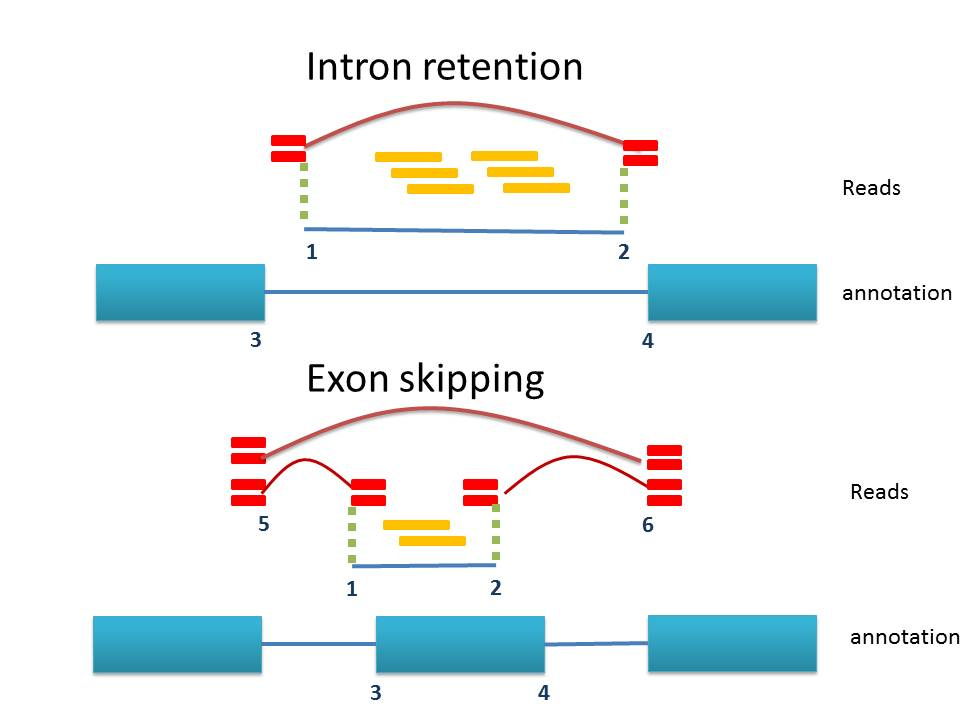
\includegraphics[width=8cm]{fig0a.jpg}
%with most subjects have dose amount between 4 and 5.}
\end{minipage}
\hspace{0.5cm} % To get a little bit of space between the figures
\begin{minipage}[b]{0.5\linewidth}
\centering
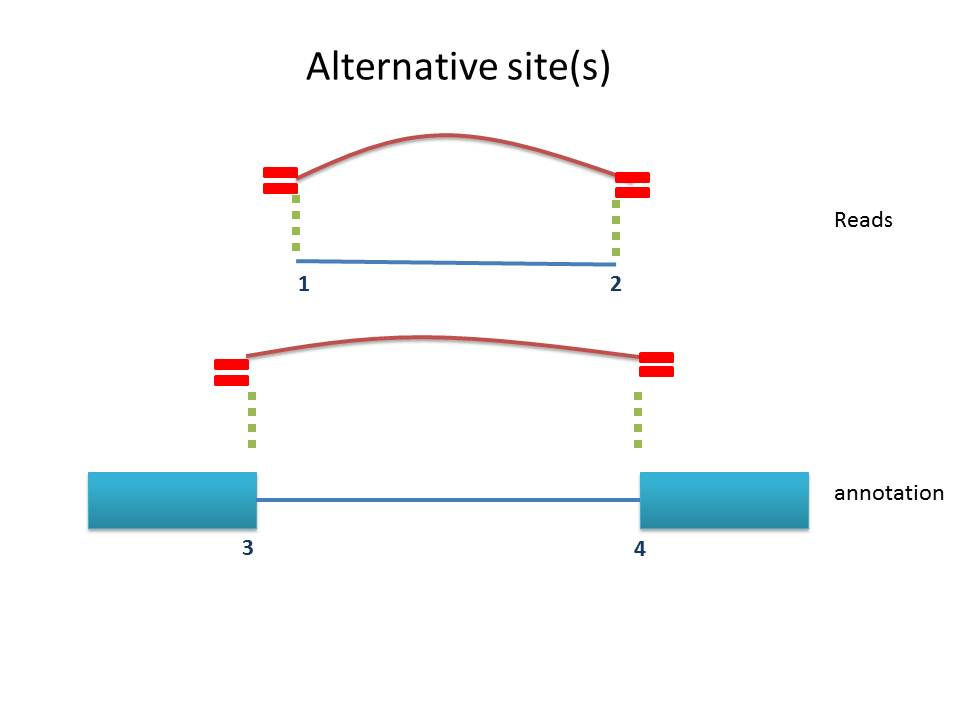
\includegraphics[width=8cm]{fig0b.jpg}
%Subjects range between 50 to 90 kilograms.}
\end{minipage}
\caption{Major splicing types inferred from reads versus annotation from gtf/gff. Nomenclature of splicing sites used in the study - 1: novel left exon boundary; 2: novel right exon boundary; 3, 5: known left exon boundary; 4, 6: known right exon boundary.}
\label{fig0}
\end{figure}

To simplify the analysis, we further divide these 
alternative splicing types to two different subtypes: 
type I and type II by comparing read information with 
the annotation files. Generally type I only consists of one intron or exon 
structure; type II consists of more than one intron or exon structures. 
More specifically, type I of exon skipping describes the alternative splicing 
events that only one exon is skipped; type II of exon skipping describes the 
events with multiple exons skipped  (Figure~\ref{fig2a}). Type I of intron retention defines the 
events that only one intron is retained; type II defines those that more than 
one intron is retained  (Figure~\ref{fig2b}). Type I of the alternative donor or acceptor covers 
those events across only one intron; while type II defines other cases  (Figure~\ref{fig2c}).
\\ \\
We use the following abbreviations: 
\begin{itemize}
	\item ri.1: type I of the intron retention.
	\item ri.2: type II of the intron retention.
	\item es.1: type I of the exon skipping.
	\item es.2: type II of the exon skipping.
	\item adleft.1: type I of the alternative donor site.
	\item adleft.2: type II of the alternative donor site.
	\item adright.1: type I of the alternative acceptor site.
	\item adright.2: type II of the alternative acceptor site.
	\item adboth.1: type I of the alternative both sites.
\item adboth.2: type II of the alternative both sites.
\end{itemize} 

\begin{figure}[ht]
\centering
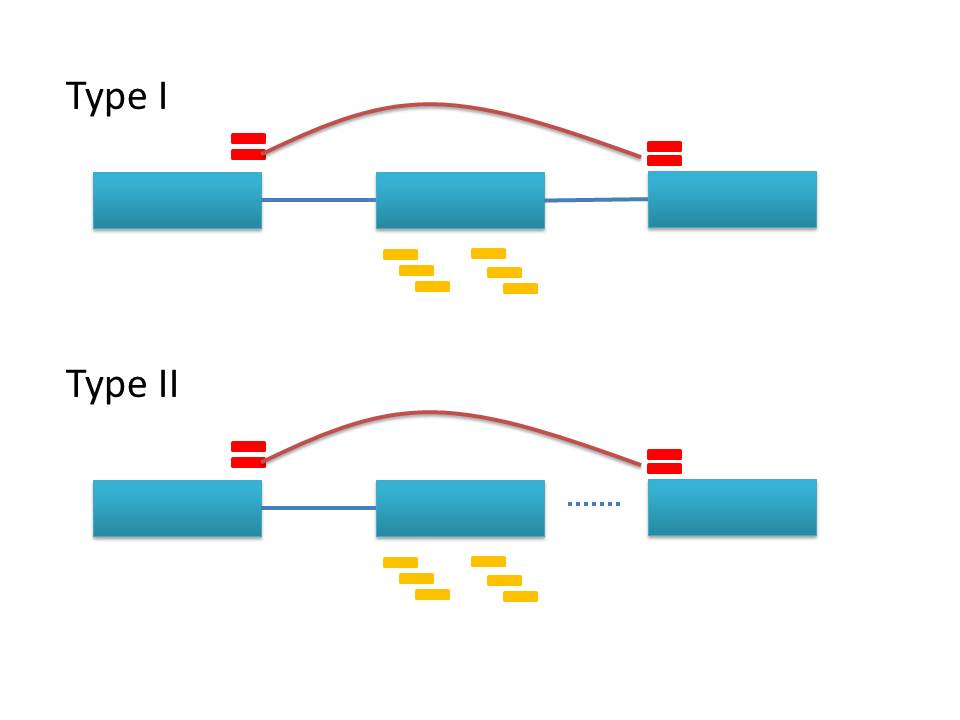
\includegraphics[scale=0.5]{fig1.jpg}
\caption{Two types of exon skipping: es.1 and es.2.}
\label{fig2a}
\end{figure}

\begin{figure}[ht]
\centering
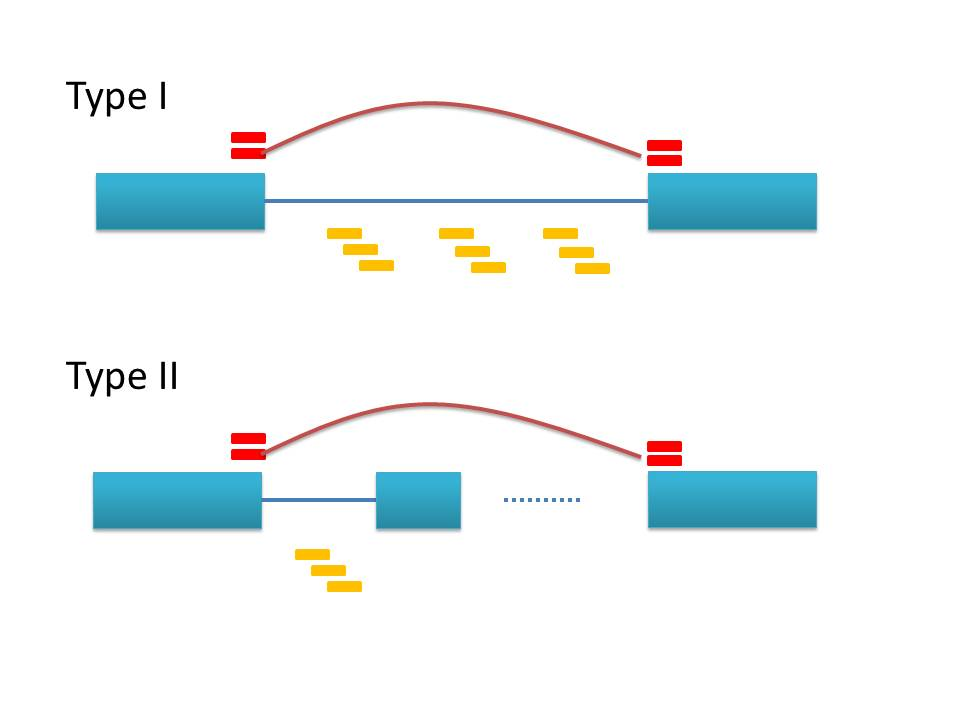
\includegraphics[scale=0.5]{fig2.jpg}
\caption{Two types of intron retention: ri.1 and ri.2.}
\label{fig2b}
\end{figure}

\begin{figure}[ht]
\centering
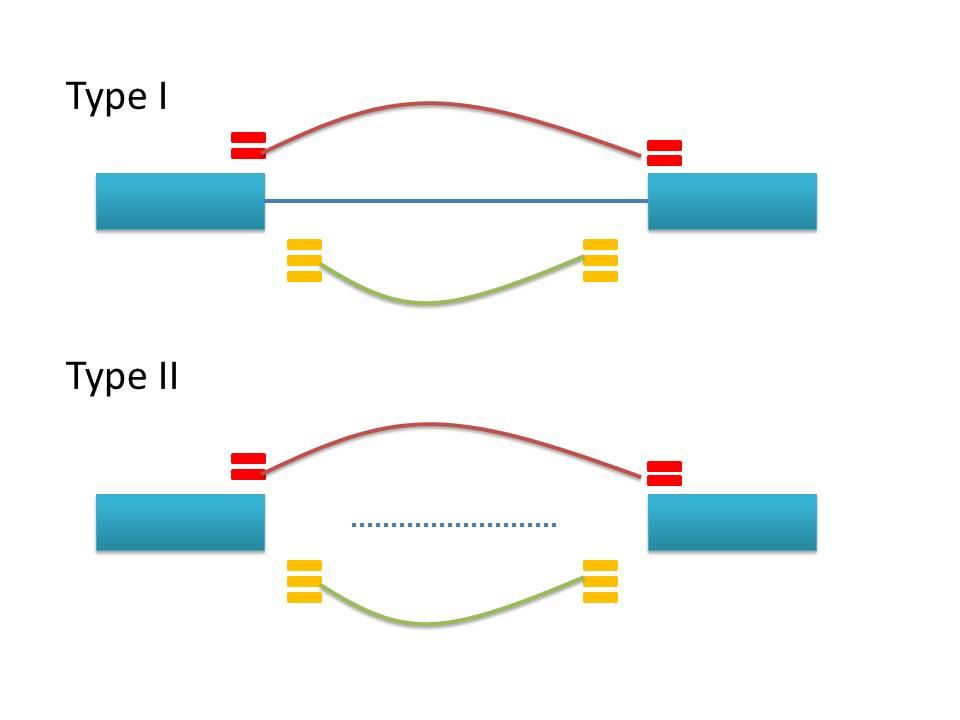
\includegraphics[scale=0.5]{fig3.jpg}
\caption{Two types of alternative both sites: adboth.1 and adboth.2.}
\label{fig2c}
\end{figure}

\section{Gene-level analysis and global-level analysis}
\subsection{Gene-level analysis}
This section describes how to analyze data for one gene or a few genes. The package requires a gtf/gff file and an alignment bam file as input and can extract the sequencing data for this gene or a few genes from one bam files (one sample) or multiple bam files (multiple samples).  The final output can either be a list object with major splicing types or a user-friendly web report.
\\ \\
The analysis at this level includes two steps: 1) creating exon\_intron structure by \texttt{translateGTF} function; 2) extracting related reads from bam file and annotating splicing types.
\\ \\
The main functions are \texttt{splicingGene}, \texttt{splicingReport}, \texttt{splicingCount}, \texttt{combineGene}, and \texttt{combineCount}. See details in the \textbf{Function description} section.
\subsection{Global-level analysis}
The analysis at this level focuses on how to globally analyze all genes for one sample or multiple samples. The package takes a gtf/gff file and an alignment bam file as input, and generates a convenient web report as output in the current working directory.

\section{Input and output}
\subsection{Annotation file: gtf/gff file}
For requirement of general format, see details at UCSC (http://genome.ucsc.edu/FAQ/FAQformat). For examples,
use \textbf{?translateGTF} to see details.
\\ \\
The annotation file should NOT have header, and start as the first line. The file
should be tab-delimited text file.
\subsection{Alignment file: bam file}
Each bam file represents one sample, generated from alignment software, such as
bowtie or tophat. Paired-end data are treated as single-end data.


\subsection{Output}
%\subsubsection{metrics}
The output columns are, 
\begin{itemize}
\item \textbf{mergeID}: the identifier for merging this splicing type across multiple samples.
      The mergeID consists of chromosome number, genomic coordinates and strand information. The genomic coordinates are the two internal boundaries of the junction reads.  
      For intron retention, the mergeID should be for an inferred intron, which is the retained intron
      for exon skipping, the mergeID should be for an inferred exon, which is the skipped exon;
      for alternative sites, the mergeID should be the gap of between two splicing junctions.
      It may or may not match the known annotation. \\ \\
      e.g., chr2:24907270-24907551\_+: 24907270 and 24907551 are site 1 and site 2 in Figure~\ref{fig0}.
\item \textbf{geneName}: the gene name from gtf/gff file. Specifically, for gtf file,
      it should be "Attributes". \\ \\
      e.g., gene\_id Pnpla7\_chr2\_+\_intron\_30: for intron retention. \\
      e.g., gene\_id LOC683722; gene\_name LOC683722; p\_id P10335; transcript\_id NM\_001101008; tss\_id TSS1868;Exon\_7: for exon skipping. \\       
\item \textbf{nonjun}: the number of non-junction reads invovled in this splicing type.
\item \textbf{jun}: the number of junction reads invovled in this splicing type.
\item \textbf{nonjun.norm}: the scaled number of non-junction reads, $(no*10^6)/(totalReadsOfBamFile*eventLength)$.
\item \textbf{jun.norm}: the scaled number of junction reads, $(no*10^6)/(totalReadsOfBamFile*readLength*2)$.
\item \textbf{ratio}: the percentage of splicing types. For intron retention, it should
be $nonjun/(jun+nonjun)$; for exon skipping, it should be $jun/(nonjun+jun)$; for alternative sites,
it should be $altersite1/(altersite1+altersite2)$.
\item \textbf{junLeftBorder}: the end coordinate of the left junction. It is site 1 in Figure~\ref{fig0}.
\item \textbf{junRightBorder}: the start coordinate of the right junction. It is site 2 in Figure~\ref{fig0}.
\item \textbf{intronStart}: the start coordinate of the intron (for intron retention). It is site 3 in intron retention of Figure~\ref{fig0}.
\item \textbf{intronEnd}: the end cooridnate of the intron (for intron retention). It is site 4 in intron retention of Figure~\ref{fig0}. 
\item \textbf{exonStart}: the start coordinate of the exon ( for exon skipping). It is site 3 in exon skipping of Figure~\ref{fig0}.
\item \textbf{exonEnd}: the end coordinate of the exon ( for exon skipping). It is site 4 in exon skipping of Figure~\ref{fig0}.
\item \textbf{count, countMax, countSum}: there are three metrics for measuring  
  alternative acceptor/donor/both site(s): count, countSum, and countMax (for alternative sites). 
  For one event of alternative site, it involves a few different sites 
  inferred from a few different junction reads. To differentiate these, 
  \textbf{count} is the number of reads for one specific site; 
  \textbf{countMax} is the number of reads for one specific site which has the 
  maximum number of junction reads; \textbf{countSum} is the number of total 
  reads for all the sites.   
\item \textbf{junLeftEndCollection}: the coordinate and reads number collection for the 5' site of all the splicing types (for alternative site).
\\ \\
  e.g., 100031\_100220,10\_14: Let's assume that the splicing event is alternative donor site, and site 2 and site4 matches in Figure~\ref{fig0} . Then 100031 and 100220 are the site 1 and site 3 (5' site), and 10 and 14 are the read number for the junction read with site1, and the junction read with site 3 respectively.
\item \textbf{junRightStartCollection}: the coordinate and reads number collection for the 3' site of all the splicing types (for alternative site).
\item \textbf{novelSplicingLink}: the novel splicing links between two exons (for alternative site).
\item \textbf{novelLeft}: the novel 5' site (for alternative site).
\item \textbf{novelRight}: the novel 3' site (for alternative site).  
\item \textbf{note}: annotation for special case. For example, some intron retention may occur inside exon.
This may happen when there are two samll exons overlapped with the third big exon.
\item \textbf{note2}: summary sentence for ratio.
\\ \\
e.g., 0.4167=100031\_100220,10\_14\_SR813\_adleft.1: \textbf{0.4167} is calculated from $10/(10+14)$; \textbf{100031, 100220} are two alternative sites for alternative donor sites; \textbf{10,14} are the read number for two alternative sites; \textbf{SR813} is the sample name for the bam file; \textbf{adleft.1} is the type I of the alternative donor site. 
\end{itemize}

\section{Function description} 
The main features of this package are 1) to translate gtf/gff file to exon\_intron structure; 2) to count the reads for exon\_intron structure; 3) to calculate and annotate the major splicing types. The first feature is implemented by \texttt{translateGTF}; the second feature requires two functions: \texttt{splicingCount} and \texttt{combineCount}. The last feature is achieved by two functions: \texttt{splicingGene} and \texttt{splicingReport}.
\subsection{Translate gtf/gff file to exon}
\subsubsection{translateGTF}
\begin{verbatim}
translateGTF(gtfFile,   
             gtfChrFormat="chr", # "Chr", "Chr0", "chr0", "1" 
             gtfGeneLabel="gene_id",
             gtfGeneValue= "g", # "g.1"
             gtfTranscriptLabel=NULL, # "Parent="  "transcript_id"                          
             exonString="exon",
             selectGenes=NULL,
             gtfColnames=c("chr", "source", "feature", "start", 
                           "end","score", "strand", "frame", 
                           "geneName"),
             geneOverlap="both", 
             exonOverlap="yes"
             )

\end{verbatim}
Translate gtf/gff file to the \texttt{GRanges}  object with gene, exon and intron structure.
It is a preprocessing tool for function \texttt{splicingGene}.
\newline  \newline
Use \texttt{? translateGTF} for details about parameters. \newline

\subsection{Count the reads for exon\_intron structure}
\subsubsection{splicingCount}
\begin{verbatim}
splicingCount(selectGene,
              bamFile = "accepted_hits.sort.bam",
              select.GRange, 
              sampleName="sample",
              sampleID=1, type="any"
              )
\end{verbatim}
Count the reads within gene, exon and intron for one gene. The selected GRange object, coming
from \texttt{translateGTF}.
\newline  \newline
Use \texttt{? splicingCount} for details about parameters. \newline

\subsubsection{combineCount}
\begin{verbatim}
combineCount(sample.list)
\end{verbatim}
Combine the results from \texttt{splicingCount} for all samples.
\newline  \newline
Use \texttt{? combineCount} for details about parameters. \newline

\subsection{Calculate and annotate the major splicing types}
\subsubsection{splicingGene}

\begin{verbatim}
splicingGene(selectGene,
                      bamFile,
                      select.GRange,
                      eventType=c("ri.1", "ri.2", "es.1", "es.2", 
                                  "adleft.1", "adleft.2", 
                                  "adright.1", "adright.2",
                                  "adboth.1", "adboth.2"),
                      sampleName="sample",
                      sampleID=1, 
                      reportSummary=TRUE,
                      minReadCounts = 10, 
                      ratioNorm=FALSE, 
                      novel="both"
                      )
\end{verbatim}
This function belongs to gene-level analysis. It only works on single gene, and helps users 
to process mutiple bam files in a few seconds. It is a convenient tool for those who do not
have access to cluster computing environment. 


\subsubsection{splicingReport}
\begin{verbatim}
splicingReport(inputData=sampleList, 
                        gtfFile, 
                        gtfChrFormat="chr", 
                        gtfGeneLabel="gene_id", 
                        gtfGeneValue="g",
                        gtfTranscriptLabel=NULL,
                        outputDir="html", 
                        eventType=c("ri.1", "ri.2", "es.1", "es.2", 
                                  "adleft.1", "adleft.2", 
                                  "adright.1", "adright.2",
                                  "adboth.1", "adboth.2"),
                         inputFile=sampleFile,
                         minReadCounts=10,                     
                         selectGenes=NULL, 
                         ratioNorm=FALSE, 
                         novel="both", 
                         parallel=FALSE, cpus=2
                        )
\end{verbatim}
This function can be either gene-level analysis or global-level anaysis dependent on the \texttt{selectGenes} parameter.
A web report will be generated in the current working directory. 
\\ \\
\textbf{Hardware requirement}: for gene-level analysis, there is no specific requirement;
for global-level analysis, this function requires a large amount of memory. Users can 
take advantage of parallel computing to speed up the analysis.

\section{Demonstration}
To illustrate how to use this package, two data sets are 
used(SRR094623 and SRR094624). The analysis pipeline includes,
1) translating gtf/gff3 to gene, exon and intron structure;
2) counting reads at the gene-level;
2) quantifying and annotating at the gene-level;
3) quantifying and annotating at the global-level.
\subsection{Data sets}
The raw data are from NCBI SRA GSE26561.
The SRR094623 is for control, and the SRR094624 is for knockout. After aligning
the raw data with tophat, we only selected the reads mapping to one gene: \emph{Pnpla3}.
\subsection{Analysis pipeline}
1. We first convert the gff3 file to gene/exon/intron structure.
%\begin{verbatim}
\begin{Schunk}
\begin{Sinput}
> options(width = 50)
> library(SplicingTypesAnno)
> mm9.pnpla7.gtfFile <- system.file("extdata", 
+     "mm9_Pnpla7.gtf", package = "SplicingTypesAnno")
> result.GRange <- translateGTF(mm9.pnpla7.gtfFile, 
+     gtfTranscriptLabel = "transcript_id")
\end{Sinput}
\begin{Soutput}
[1] "Done..."
\end{Soutput}
\end{Schunk}
%\end{verbatim}
2. Then we count the reads for exon and intron respectively
%\begin{verbatim}
\begin{Schunk}
\begin{Sinput}
> bam.1 <- system.file("extdata", "liver_ctr.sort.bam", 
+     package = "SplicingTypesAnno")
> bam.2 <- system.file("extdata", "liver_ko.sort.bam", 
+     package = "SplicingTypesAnno")
> selectGene <- "Pnpla7"
> sample1.c <- splicingCount(selectGene, 
+     bam.1, result.GRange, sampleName = "liver_ctr", 
+     sampleID = 1)
\end{Sinput}
\begin{Soutput}
[1] "GENE - Pnpla7 are processed..."
[1] "some chrNo in bam file are NOT in gtf/gff3 file! The unmatched data will be overlooked..."
\end{Soutput}
\begin{Sinput}
> sample2.c <- splicingCount(selectGene, 
+     bam.2, result.GRange, sampleName = "liver_ko", 
+     sampleID = 2)
\end{Sinput}
\begin{Soutput}
[1] "GENE - Pnpla7 are processed..."
[1] "some chrNo in bam file are NOT in gtf/gff3 file! The unmatched data will be overlooked..."
\end{Soutput}
\end{Schunk}
%\end{verbatim}
3. To compare different samples, we combine all the results.
%\begin{verbatim}
\begin{Schunk}
\begin{Sinput}
> sList.c <- list(sample1.c, sample2.c)
> ccount <- combineCount(sList.c)
\end{Sinput}
\end{Schunk}
%\end{verbatim}
4. In addition, we can quantify and annotate the major splicing types at the gene-level.
\begin{verbatim}
selectGene <- c("Pnpla7")
sample1 <- splicingGene(selectGene, bam.1, result.GRange,
                        sampleName="liver_ctr", sampleID=1
                        )

sample2 <- splicingGene(selectGene, bamFile2, result.GRange,
                        sampleName="liver_KO", sampleID=2
                        )

sList <- list(sample1$type, sample2$type)
ri.1 <- combineGene(sList, splicingEvents="ri.1", selectGenes)
ri.2 <- combineGene(sList, splicingEvents="ri.2", selectGenes)
es.1 <- combineGene(sList, splicingEvents="es.1", selectGenes)
es.2 <- combineGene(sList, splicingEvents="es.2", selectGenes)
adleft.1 <- combineGene(sList, splicingEvents="adleft.1", selectGenes)
adleft.2 <- combineGene(sList, splicingEvents="adleft.2", selectGenes)
adright.1 <- combineGene(sList, splicingEvents="adright.1", selectGenes)
adright.2 <- combineGene(sList, splicingEvents="adright.2", selectGenes)
adboth.1 <- combineGene(sList, splicingEvents="adboth.1", selectGenes)
adboth.2 <- combineGene(sList, splicingEvents="adboth.2", selectGenes)
\end{verbatim}
5. Finally we can generate a user-friendly web report.
\begin{verbatim}
sampleList <- list(SampleName=c("liver_ctr", "liver_ko"),
                    BamFiles=c(bam.1, bam.2),
                    SampleID=c(1,2)
                     )
splicingReport(inputData=sampleList, 
               gtfFile=mm9.pnpla7.gtfFile, 
               selectGenes=c("Pnpla7"))
\end{verbatim}
6. The bed files in the report can be visualized in IGV. 
\end{document}




